\documentclass[11pt]{article}

\usepackage[final]{acl}
\usepackage{times}
\usepackage{latexsym}
\usepackage[utf8]{inputenc}
\usepackage[T1]{fontenc}
\usepackage{booktabs}
\usepackage{amsmath}
\usepackage{amssymb}
\usepackage{graphicx}
\usepackage{microtype}

\newcommand{\linkding}{\textsc{Linkding}}
\newcommand{\expel}{\textsc{ExpeL}}
\newcommand{\webcoevo}{\textsc{WebCoEvo}}
\newcommand{\sr}{\mathrm{SR}}

\title{\webcoevo{}: Adversarial Co-Evolution for Web-Agent Reflection Rules\\Capability-Targeted Website Drift on \linkding{}}

\author{
  Chenming Ge, Chengyang Shi, Yifei Xu, Yuxiang Yang, Binglin Zhong \\
  University of Michigan \\
  \texttt{\{gecm, chengysh, xuyifei, yyxxyj, tozenith\}@umich.edu}
}

\begin{document}

\maketitle

\begin{abstract}
Web agents often fail when a website changes in ways that preserve the user's goal but disrupt learned interface shortcuts. We present \webcoevo{}, a single-site but end-to-end auditable loop for generating capability-targeted website drift and testing compact reflection rules. The loop profiles failures, builds fresh \linkding{} website overlays, mines matched trajectory transitions, edits a small reflection rulebook, and evaluates the resulting policy with prompt-injection evidence recorded in trace JSONL. The upgraded WebCoEvo evidence covers three website versions: \linkding{} V1.45.0, a moderately modified website V2, and a harder generated website suite V3 over seven drift categories. On the 68 training tasks from \linkding{} V1.45.0, \expel{}-style rules raise Qwen3-VL success from \(9/68=13.2\%\) to \(56/68=82.4\%\). Under website V2, R1 reflection rules improve over \expel{}-style prompting from \(60/68=88.2\%\) to \(67/68=98.5\%\) on the training tasks and from \(114/167=68.3\%\) to \(143/167=85.6\%\) on the held-out validation tasks. On website V3, \expel{}-style prompting collapses to \(8/68=11.8\%\) on the training tasks and \(66/167=39.5\%\) on the held-out validation tasks, while R1 reaches \(65/68=95.6\%\) and \(97/167=58.1\%\). A GPT-5.4-assisted R2 update ties R1 on the held-out validation tasks but does not improve the training tasks, showing that iterative reflection is useful but not monotonic. We claim auditable \linkding{} robustness improvement from compact reflection rules, not universal web-agent robustness.

\end{abstract}

\section{Introduction}

Web-agent benchmarks are becoming more realistic, but most still treat website change as a fixed nuisance: choose a set of versions or perturbations, run an agent, and report success rate. That protocol measures brittleness, yet it does not answer the design question that appears after each evaluation. Once an agent has a strong rulebook, which website changes still expose its capability boundary, and how should the next rule update be selected?

This question matters for reflection-based agents. A reflection rule such as ``preserve a login redirect'' or ``stop when the target state is already visible'' only helps if the benchmark contains valid situations where that behavior is required. If generated websites are too easy, they provide no learning signal. If they are broken, failures cannot support a rule. \webcoevo{} studies the middle ground: use the current agent as a solver, generate websites that target its observed frontier, and mine small cross-version reflection rules from paired trajectory evidence.

We instantiate this loop on \linkding{}, a self-hosted bookmark manager with deterministic local deployment and code-level website overlays. The agent is Qwen3-VL in a BrowserGym/AgentLab/UI-TARS stack. The base policy can receive \expel{} task-experience rules distilled from earlier trajectories, while the cross-version layer injects compact reflection rules about how to adapt when the website changes. This separation is important. \expel{} rules tell the agent what helped on related tasks; cross-version reflection rules tell it how to preserve task intent across a shifted interface.

The upgraded WebCoEvo evidence has three website versions. The first is \linkding{} V1.45.0, the original release. The second is a moderately modified website V2 that tests whether R1 reflection rules improve over \expel{}-style prompting under moderate website drift. The third is a harder generated website suite V3 with seven drift categories: \texttt{access}, \texttt{surface}, \texttt{content}, \texttt{runtime}, \texttt{process}, \texttt{structural}, and \texttt{functional}. Website V3 is the primary stress test because \expel{}-style prompting collapses there even when it performs well on \linkding{} V1.45.0 and website V2.

The main empirical result is sharper than in the earlier draft. On the 68 training tasks from \linkding{} V1.45.0, \expel{}-style rules raise success from \(9/68=13.2\%\) to \(56/68=82.4\%\). On website V2, R1 reflection rules improve over \expel{}-style prompting from \(60/68=88.2\%\) to \(67/68=98.5\%\) on the training tasks and from \(114/167=68.3\%\) to \(143/167=85.6\%\) on the held-out validation tasks. On website V3, however, \expel{}-style prompting drops to \(8/68=11.8\%\) on the training tasks and \(66/167=39.5\%\) on the held-out validation tasks. R1 recovers most of the training split, reaching \(65/68=95.6\%\), and transfers to the held-out validation tasks at \(97/167=58.1\%\). R4, a GPT-5.4-assisted update built from transition evidence, ties R1 on the held-out validation tasks but reaches only \(60/68=88.2\%\) on the training tasks, so iterative reflection is useful but not monotonic.

This paper makes three contributions.
\begin{enumerate}
\item We formulate a capability-targeted adversarial co-evolution protocol for web-agent reflection rules: profile current failures, generate drifted websites at the boundary, audit task validity, mine behavior gaps, and promote only compact rule updates that survive validation.
\item We materialize the protocol in \webcoevo{}, a standalone \linkding{} runner with explicit task normalization, reset logic, prompt construction, rulebook selection, and legacy eval/trace JSONL export.
\item We report the upgraded evidence across \linkding{} V1.45.0, website V2, and website V3: \expel{}-style rules help on the original site, but compact reflection rules are what preserve performance under generated website drift, with R1 strongest on the training tasks under website V3 and R1/R4 tied on the held-out validation tasks under website V3.
\end{enumerate}

The claim boundary is deliberately narrow. We do not claim universal web-agent robustness, nor that later reflection-rule versions always improve. The evidence is single-site, and several drift families remain difficult on the held-out validation tasks under website V3. The contribution is an auditable loop that turns those failures into the next environment and rule-design targets.

\section{Related work}

\paragraph{From static web tasks to version-aware evaluation.}
Web-agent evaluation is moving from frozen, single-version tasks toward settings that better approximate deployment. Early benchmarks made browser control measurable with reproducible websites, DOM observations, screenshots, and action traces~\citep{zhou2023webarena,deng2023mind2web,koh2024visualwebarena}. Newer benchmarks add live content, deterministic replicas of real websites, long-horizon chores, and user-centered assistance where instructions can be ambiguous or evolve over time~\citep{yuan2024webcanvas,real2025,webchorearena2025,realwebassist2025}. This shift reflects a broader concern that apparent progress can be inflated by contamination, stale benchmarks, and weak agreement with human judgments~\citep{xue2025illusion}. Time-aware evaluation makes the issue especially clear: agents tuned on one web design may fail across historical interface versions~\citep{timewarp2026}. \webcoevo{} follows this version-aware direction, but treats website versions as a design variable rather than only a fixed test distribution.

\paragraph{Website evolution as task-semantic drift.}
Website change is not merely cosmetic. A valid task can keep the same user goal while changing the entry point, readiness timing, labels, workflow checkpoints, route equivalence, or login return behavior. Web-evolution and testing work already separate superficial page differences from semantic structure, dynamic UI state, visual presentation, workflow order, and authentication hazards~\citep{shao2021webevo,mesbah2012crawling,macchi2021imagebased,sanchez2011workflow,jonker2018shepherd}. Recent interface-for-agent work takes the complementary route of exposing semantic component interfaces or structured GUI knowledge so agents depend less on brittle visual shortcuts~\citep{ci4a2026,graphpilot2026}. Our drift labels---access, surface, content, runtime, process, structural, and functional---are therefore an operational language for valid completion-path changes, not a universal taxonomy of web evolution.

\paragraph{Experience loops for self-evolving agents.}
LLM-agent research is also shifting from one-shot prompting toward reusable experience. Reflection and experiential-learning methods convert trajectories into natural-language memories or rules~\citep{shinn2023reflexion,zhao2023expel}. Recent self-evolving-agent work broadens this pattern to memory, tools, policies, architectures, user interaction, and multi-agent feedback~\citep{gao2025selfevolvingagents}. In practical systems, the same trend appears as interaction-derived data, backward construction of instructions, distilled strategic principles, and policy updates from experience rather than static supervision alone~\citep{learnbyinteract2025,wu2025evolver,liang2025sage,comas2025}. \webcoevo{} uses this idea narrowly: the base web agent remains fixed, while paired control/drift traces update a compact cross-version reflection rulebook.

\paragraph{Adaptive environments and agent-environment co-evolution.}
A parallel line of work treats environments as active curricula rather than passive test sets. Unsupervised environment design, replay-guided adversarial design, and compositional environment generation all use the learner's current capability to decide which tasks should be generated or replayed next~\citep{dennis2020paired,jiang2021replayguided,gur2021code}. Newer LLM-agent work extends this idea with synthetic interaction data and generative simulators that produce tasks near the agent's useful difficulty frontier~\citep{learnbyinteract2025,genenv2025}. \webcoevo{} brings this co-evolutionary view to web-agent robustness under stricter constraints: each generated \linkding{} overlay must boot, preserve evaluator semantics, remain manually solvable, and expose a meaningful behavioral failure rather than an infrastructure artifact.

\paragraph{Positioning.}
These lines leave a missing middle layer. Version-aware benchmarks show that web-agent success is unstable across interface change; web-evolution work explains why such change is semantic; self-evolving-agent work shows how experience can become reusable guidance; and adaptive environment generation shows how the next task distribution can target an agent's frontier. \webcoevo{} connects them in one auditable loop: profile failures, generate valid website drift, mine paired trajectories, update compact reflection rules, and test whether the update preserves earlier successes.

\section{Methodology}

\subsection{Adversarial Co-Evolution Loop}

\webcoevo{} treats website generation and reflection-rule learning as a closed loop. At round \(k\), a web agent with a fixed base prompt and an optional cross-version rulebook is evaluated on a control website and on generated website variants that preserve the user goal. The resulting trajectories are converted into a capability profile:
\[
\begin{gathered}
\texttt{can\_do},\ \texttt{borderline},\ \texttt{cannot\_do},\\
\texttt{control\_unstable},\ \texttt{invalid}.
\end{gathered}
\]
We also compute paired transitions between a reference run and a candidate run:
\(\texttt{both\_success}\), \(\texttt{saved}\), \(\texttt{lost}\), and \(\texttt{both\_fail}\). The \texttt{saved} rows show which rules help; \texttt{lost} rows are no-regression counterexamples; and \texttt{both\_fail} rows define the next capability frontier.

The loop has two update paths. The environment path generates a harder website when a slice is saturated by the current rulebook. The rule path mines behavior gaps when the website is valid and failures are concentrated in recoverable agent behavior. A rule update is accepted only when it remains compact, avoids task-id-specific overfitting, preserves successful behaviors, and passes coverage checks on the benchmark task schema.

\subsection{Standalone WebCoEvo Runner}

The upgraded experiments use a standalone \linkding{} runner rather than the older multi-harness research stack. The runner has four benchmark-facing stages. First, it loads training-task or held-out-validation JSON rows and normalizes each row into a stable schema with fields such as \texttt{task\_id}, \texttt{source\_task\_id}, \texttt{drift\_type}, \texttt{variant}, \texttt{family}, \texttt{version}, and \texttt{start\_url}. Second, it launches the requested website version, resets seed data, handles localhost login and redirect recovery, and compiles each row into a BrowserGym task. Third, it builds the agent prompt from separated blocks: the task observation and goal, an optional \expel{} task-experience block, and an optional reflection-rule adaptation block. Fourth, it exports eval and trace JSONL so earlier analysis tools can read the new runs.

This separation prevents a common ambiguity in reflection-rule experiments. A rulebook file can exist on disk without actually being injected into the agent prompt. The WebCoEvo traces therefore record \texttt{injected\_rule\_ids} for the \expel{} layer and \texttt{cross\_version\_reflection\_rule\_ids} for the reflection-rule layer separately, along with the selected rulebook path, selection context, miss reasons, and reset-time errors. The website V3 headline runs are interpreted only through this trace-audited path.

\subsection{Website Versions and Drift Taxonomy}

All websites are derived from \linkding{} v1.45.0. \linkding{} V1.45.0 is the unmodified release. Website V2 is a moderately modified generated drift suite used to test whether R1 reflection rules transfer beyond the original site. Website V3 is the harder validation layer and contains seven drift labels:
\[
\begin{gathered}
\{\texttt{access},\texttt{surface},\texttt{content},\texttt{runtime},\\
\texttt{process},\texttt{structural},\texttt{functional}\}.
\end{gathered}
\]
The labels are operational. \texttt{access} shifts authentication or redirect preservation. \texttt{surface} changes visual framing and salience. \texttt{content} changes labels, placeholders, or nearby copy while preserving the data model. \texttt{runtime} changes readiness timing. \texttt{process} changes visible checkpoints in a workflow. \texttt{structural} regroups navigation affordances or route entrypoints. \texttt{functional} changes exposed feature affordances or route equivalence while keeping the task evaluable from visible state. This completion-path view is grounded in prior work on semantic web evolution, GUI properties, dynamic Ajax state changes, workflow testing, and heterogeneous login flows~\citep{shao2021webevo,macchi2021imagebased,mesbah2012crawling,sanchez2011workflow,jonker2018shepherd}.

Each generated website must pass design gates before it is used for rule mining: it should break one primary agent assumption, keep the semantic user goal unchanged, remain manually solvable, and preserve evaluator validity. Failures caused by reset, parser, port, or evaluator problems are labeled as infrastructure issues rather than rule-learning evidence.

\subsection{Rulebooks and Reflection Updates}

\expel{} rules are task-experience rules induced from failed-then-success episodes. They often contain concrete operational details such as known credentials, target pages, and completion cues. Reflection rules are intentionally compact and scoped to drift patterns rather than individual row ids.

The main reflection-rule sets are successive rule-revision rounds obtained by iteratively reflecting on observed failures:
\begin{itemize}
\item \textbf{R1:} the strongest robust rule set in the upgraded results. It emphasizes login-next preservation, stale-bid recovery, direct route fallback, finalization when target evidence is already visible, collapsed-navigation recovery, and non-interactive element rejection.
\item \textbf{R4:} a GPT-5.4-assisted update derived from R1 transition evidence. It edits two rules without adding or dropping rules, targeting login-next preservation and finalization when URL, query, heading, or redirected destination already proves completion.
\item \textbf{R2:} a staged repair candidate that strengthens access and surface recovery but loses held-out robustness on website V3.
\item \textbf{R3:} a selective merge candidate that improves over \expel{}-style rules on website V3 but does not dominate R1.
\end{itemize}

The R4 pipeline illustrates the WebCoEvo rule path. Training-task matched transitions from website V2 with R1 to website V3 with R1 contain 65 \texttt{both\_success}, 2 \texttt{lost}, 0 \texttt{saved}, and 1 \texttt{both\_fail} case. The candidate generation stage compresses these cases into constrained edit proposals, then deterministic verification checks the rulebook schema and task coverage. The resulting R4 candidate covers \(68/68\) training-task rows, but its evaluation shows why promotion cannot rely on plausibility alone: it ties R1 on the held-out validation tasks under website V3 yet is weaker than R1 on the training tasks under website V3.

\subsection{Evaluation Slices and Metrics}

We evaluate two task banks. The training split has 68 rows and is near the rule-mining distribution. The held-out validation split has 167 rows and covers unseen task families. For a slice \(S\), success rate is
\[
\sr(S)=\frac{1}{|S|}\sum_{x \in S}\mathbf{1}[\mathrm{success}(x)].
\]
We report per-drift rates, aggregate rates, and cross-version comparisons across website versions. The agent configuration is Qwen/Qwen3-VL-30B-A3B-Instruct with visual input enabled, \texttt{MAX\_STEPS}=30, and \texttt{MAX\_TOKENS}=300, using the \texttt{vl\_action\_reflection} mode through an OpenAI-compatible endpoint.

\subsection{Claim Boundary}

The upgraded method supports three claims. First, \expel{} task-experience rules are valuable on the original site but lose robustness under harder website drift. Second, compact reflection rules recover much of that lost performance and transfer to the held-out validation tasks. Third, rule iteration is not monotonic: R4 is evidence-aware and trace-audited, but R1 remains the strongest rule set on the training tasks under website V3. The method does not yet establish robustness beyond \linkding{} or prove that a single rulebook dominates every drift family.

\section{\linkding{} Experimental Setup}

\subsection{Task Banks}

The training split is the calibration anchor for WebCoEvo. It contains 68 rows over task families chosen because they expose failures in login redirects, filtered views, prefilled forms, and navigation under website drift. We treat it as training-like because the reflection-rule loop is diagnosed and edited near this distribution. The held-out validation split contains 167 rows over unseen task families. We report the two task banks separately because averaging them would mix a rule-mining slice with a transfer slice.

\subsection{Website Suites}

The upgraded evaluation uses three \linkding{} website suites.
\begin{itemize}
\item \textbf{\linkding{} V1.45.0:} the original unmodified \linkding{} release, used to measure the value of no rules versus \expel{} task-experience rules.
\item \textbf{Website V2:} a moderately modified generated website suite, used to compare \expel{}-style prompting with R1 reflection rules.
\item \textbf{Website V3:} the harder generated website suite, with seven release-grounded website overlays for \texttt{access}, \texttt{surface}, \texttt{content}, \texttt{runtime}, \texttt{process}, \texttt{structural}, and \texttt{functional} drift.
\end{itemize}

Website V2 is useful because it shows that R1 improves transfer before the harder generated website suite. Website V3 is useful because it exposes a sharper capability boundary: \expel{}-style prompting remains strong on earlier websites but drops sharply under this harder generated suite.

\subsection{Agent and Prompt Conditions}

All headline runs use Qwen/Qwen3-VL-30B-A3B-Instruct with visual input enabled, \texttt{vl\_action\_reflection} agent mode, \texttt{MAX\_STEPS}=30, and \texttt{MAX\_TOKENS}=300. The prompt can contain three separated sources of information: the current observation and goal, \expel{} task-experience rules, and reflection rules. The \linkding{} V1.45.0 matrix compares no rules with \expel{}-style rules. The website V2 matrix compares \expel{}-style rules with R1 reflection rules. The website V3 matrix compares \expel{}-style rules with R1--R4 reflection rules.

\subsection{Rulebook Selection and Auditing}

The website V3 comparison evaluates each reflection-rule set as a compact whole policy with coarse drift matching. It does not use source-task-id gating in the headline comparison. The runner records prompt injection explicitly: \texttt{injected\_rule\_ids} for \expel{} rules and \texttt{cross\_version\_reflection\_rule\_ids} for reflection rules. It also records rulebook paths, selection context, miss reasons, and reset-time errors. This lets the results be interpreted as rule-conditioned runs rather than as silent no-rule reruns.

\subsection{Provenance}

The upgraded data come from completed WebCoEvo reports generated on April 17-18, 2026 under \texttt{/home/gecm/WebCoEvo}. The key report files are the website V3 reflection-rule matrix report, the UMich Qwen3-VL rule-comparison report, the website-version line report, and the GPT-5.4 R4 reflection-hardening report. Appendix Table~\ref{tab:artifact_paths} lists the local artifacts used to update the paper.

\section{Results}

\begin{table*}[t]
\centering
\small
\begin{minipage}{0.48\textwidth}
\centering
\textbf{Training tasks}\\[2pt]
\begin{tabular}{lrrr}
\toprule
Website & No rules & \expel{}-style & Reflection \\
\midrule
V1.45.0 & 9/68 & 56/68 & -- \\
V2 & -- & 60/68 & 67/68 \\
V3 & -- & 8/68 & 65/68 \\
\bottomrule
\end{tabular}
\end{minipage}
\hfill
\begin{minipage}{0.48\textwidth}
\centering
\textbf{Held-out validation tasks}\\[2pt]
\begin{tabular}{lrrr}
\toprule
Website & No rules & \expel{}-style & Reflection \\
\midrule
V1.45.0 & 133/167 & 124/167 & -- \\
V2 & -- & 114/167 & 143/167 \\
V3 & -- & 66/167 & 97/167 \\
\bottomrule
\end{tabular}
\end{minipage}
\caption{Overall success counts across website versions. \expel{}-style rules help on \linkding{} V1.45.0 but degrade under harder website drift. Reflection rules remain stronger on the generated website suites. Detailed per-drift results for R1--R4 on website V3 are reported in Appendix Tables~\ref{tab:training_v3_appendix} and~\ref{tab:heldout_v3_appendix}.}
\label{tab:website_version_summary}
\end{table*}

\begin{figure*}[t]
\centering
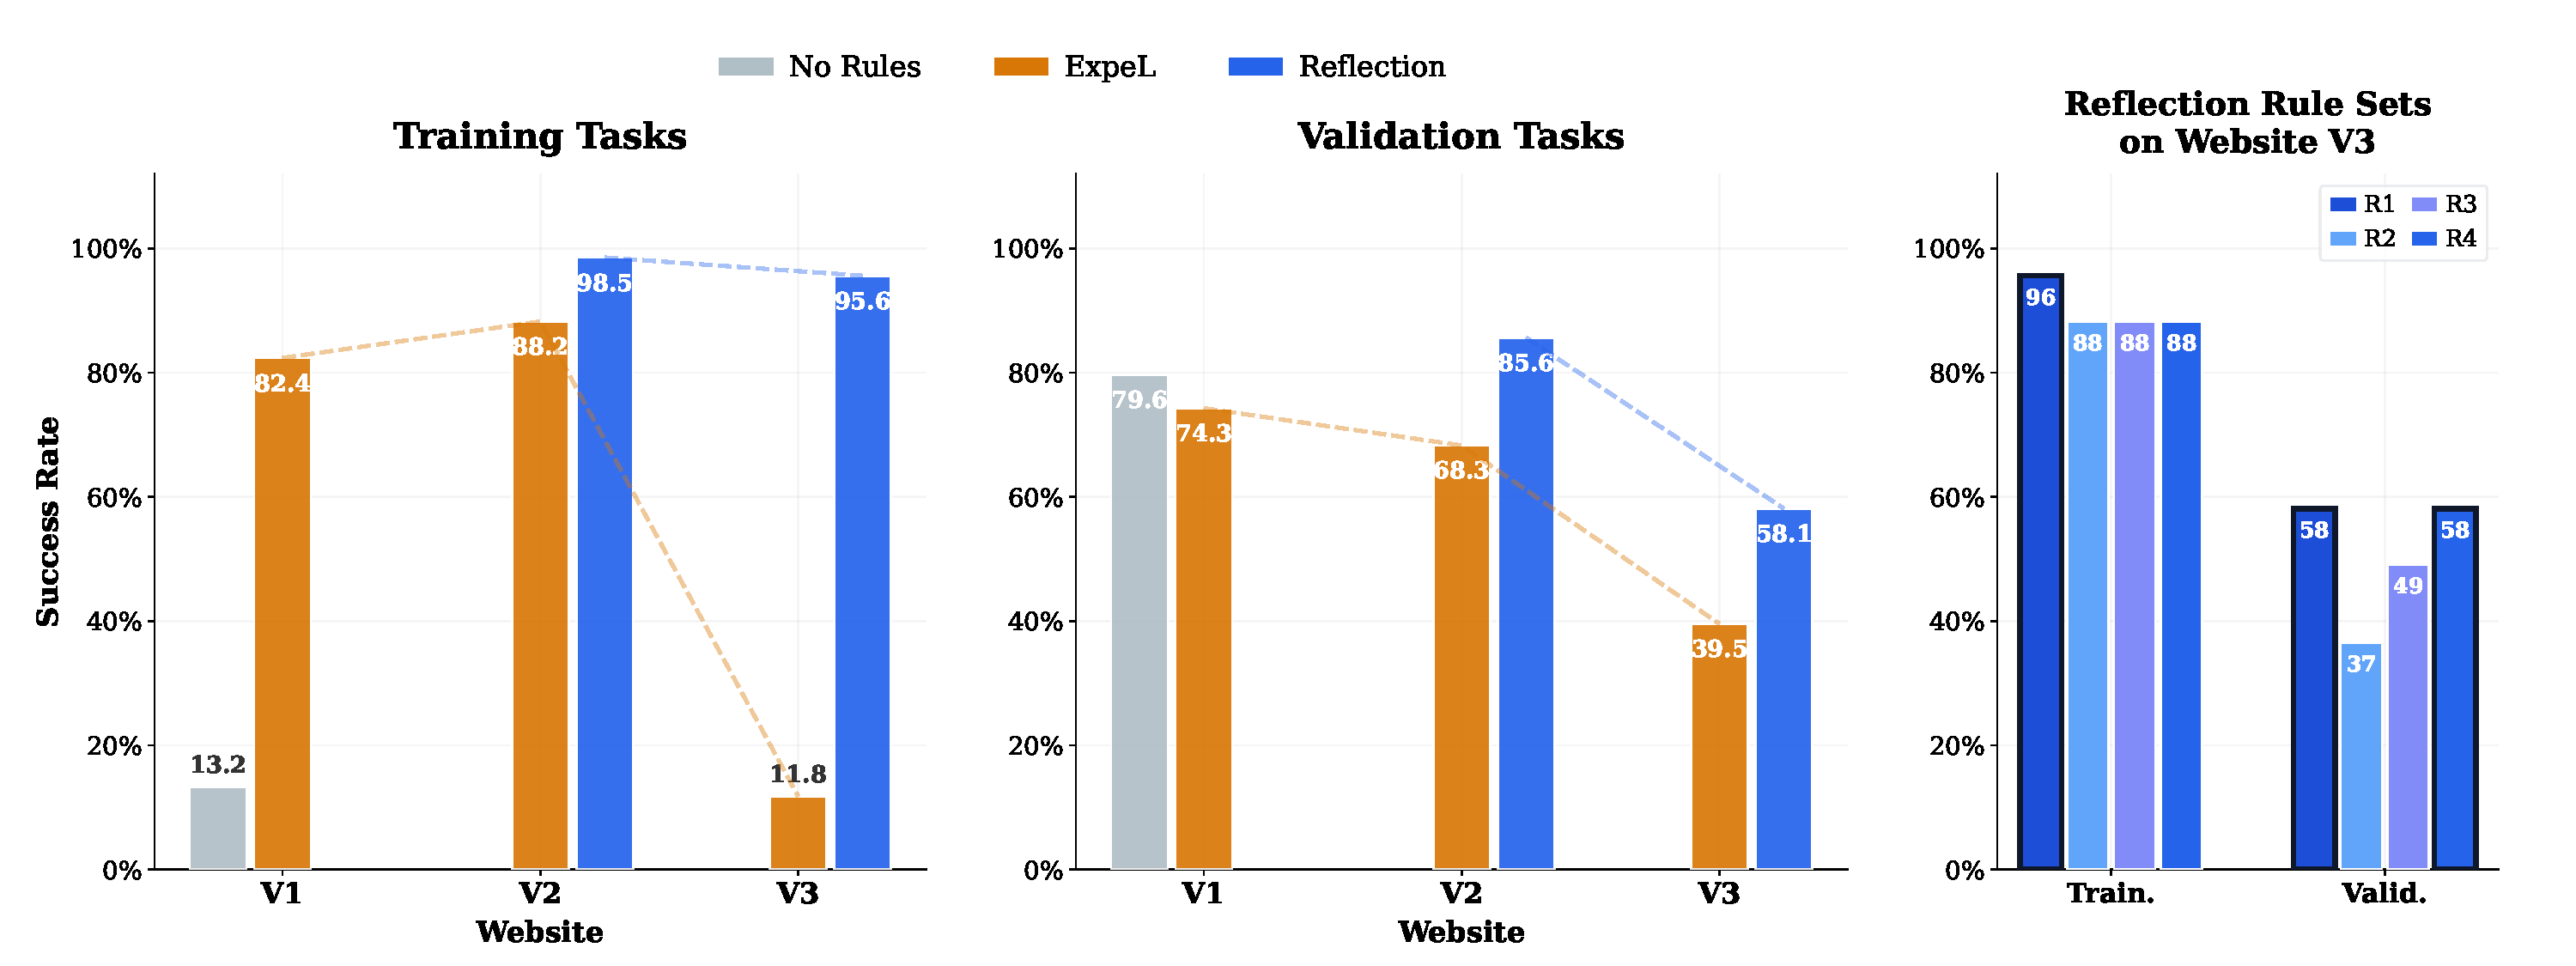
\includegraphics[width=\textwidth]{output/poster_fig_a_hero.pdf}
\caption{Headline robustness results across website versions. The left and middle panels compare no rules, \expel{}-style rules, and the strongest available reflection-rule condition on the training and held-out validation tasks. The right panel isolates the website V3 reflection-rule sets R1--R4, showing that later rule revisions are not monotonically better.}
\label{fig:website_version_overview}
\end{figure*}

\begin{table}[t]
\centering
\small
\begin{tabular}{lcc}
\toprule
Rules & Training & Held-out \\
\midrule
R1 & 65/68 (95.6\%) & 97/167 (58.1\%) \\
R2 & 60/68 (88.2\%) & 97/167 (58.1\%) \\
R3 & 60/68 (88.2\%) & 61/167 (36.5\%) \\
R4 & 60/68 (88.2\%) & 82/167 (49.1\%) \\
\bottomrule
\end{tabular}
\caption{Overall website V3 success for successive reflection-rule sets. R1--R4 are obtained through iterative reflection on observed failures and rule revision; detailed per-drift counts are deferred to Appendix Tables~\ref{tab:training_v3_appendix} and~\ref{tab:heldout_v3_appendix}.}
\label{tab:v3_reflection_overall}
\end{table}


\paragraph{Experimental setting.}
We evaluate a fixed multimodal web agent on a self-hosted bookmark-management website under three conditions: no retrieved rules, \expel{}-style rules~\citep{zhao2023expel}, and \expel{}-style rules augmented with reflection rules. The evaluation uses 68 training tasks for diagnosing rule behavior and 167 held-out validation tasks for testing transfer to unseen task families. We report task success rate on \linkding{} V1.45.0, on a moderately modified website V2, and on a harder generated website suite V3 that changes access, visual presentation, content, timing, workflow, navigation structure, and feature affordances while preserving the user goal. For website V3, R1--R4 denote successive reflection-rule sets obtained through iterative reflection on observed failures and rule revision.

\subsection{\expel{}-Style Rules Help, but Do Not Fully Transfer}

On \linkding{} V1.45.0, \expel{}-style rules provide a strong training-task gain: success increases from \(13.2\%\) without rules to \(82.4\%\) with retrieved \expel{}-style rules. This confirms that reusable experience is a meaningful starting point rather than a weak baseline. The same rules, however, do not uniformly improve held-out behavior. On held-out validation tasks from \linkding{} V1.45.0, success changes from \(79.6\%\) without rules to \(74.3\%\) with \expel{}-style rules. This motivates separating training tasks from held-out validation tasks instead of reporting a single averaged score.

\subsection{Reflection Rules Help Under Moderate Website Drift}

We next test whether reflection rules add value when the website changes but the task goals remain the same. On website V2, adding reflection rules improves the training tasks from \(88.2\%\) to \(98.5\%\), and improves the held-out validation tasks from \(68.3\%\) to \(85.6\%\) (Table~\ref{tab:website_version_summary} and Figure~\ref{fig:website_version_overview}). Since the model, tasks, website version, and \expel{}-style rules are held fixed, these gains isolate the benefit of rules that describe how to preserve intent across interface changes.

\subsection{Website V3 Exposes the Robustness Gap}

The harder generated website suite V3 creates the main robustness stress test. With \expel{}-style rules alone, success drops to \(11.8\%\) on the training tasks. The strongest reflection-rule set recovers performance to \(95.6\%\), while three alternative rule sets reach \(88.2\%\) (Table~\ref{tab:v3_reflection_overall}). Figure~\ref{fig:v3_drift_rule_profile} shows that the recovery is broad across drift families rather than coming from a single easy bucket. This large gap shows that robustness under website drift is not obtained simply by adding more task-level guidance; the useful rules are those that explicitly describe how to recover from changed navigation paths, delayed readiness, changed labels, and shifted workflow cues.

The held-out validation tasks remain substantially harder. \expel{}-style rules alone reach \(39.5\%\). The two strongest reflection-rule sets, R1 and R4, reach \(58.1\%\), while weaker variants R3 and R2 reach \(49.1\%\) and \(36.5\%\). Thus, reflection rules improve transfer under harder drift, but the gains are uneven: a plausible rule update can improve one family of failures while regressing another.

\subsection{Rule Updates Are Useful but Non-Monotonic}

The detailed website V3 matrices in Appendix Tables~\ref{tab:training_v3_appendix} and~\ref{tab:heldout_v3_appendix}, summarized visually in Figure~\ref{fig:v3_reflection_iteration} and Figure~\ref{fig:v3_drift_rule_profile}, show that the best aggregate reflection-rule set is not simply the most recent edit. One evidence-based update improves several held-out drift categories, including authentication-related, visual, content, and timing changes, but loses ground on workflow and feature-affordance changes. The aggregate tie on the held-out validation tasks therefore hides a real tradeoff between different recovery behaviors.

This pattern supports the main design choice in \webcoevo{}: rule generation, verification, and promotion should be separate stages. Matched trajectories can suggest useful edits, but an edit should not be promoted only because it is plausible or locally evidence-grounded. It must also preserve previously successful behaviors under the same website-drift distribution.

\subsection{Failure Analysis: Why Iterative Reflection Degrades Held-Out Generalization}
\label{sec:failure_analysis}

The per-drift breakdown in Appendix Tables~\ref{tab:training_v3_appendix} and~\ref{tab:heldout_v3_appendix} exposes a sharp asymmetry between training and held-out behavior. On the 68 training tasks, successive rule sets differ modestly: R1 reaches \(65/68\) and R2--R4 each reach \(60/68\). On the 167 held-out tasks, the same transition produces a collapse: R1 achieves \(97/167=58.1\%\), R2 falls to \(61/167=36.5\%\)---\emph{below} the \expel{}-only baseline of \(66/167=39.5\%\)---and R3 and R4 partially recover to \(82/167=49.1\%\) and \(97/167=58.1\%\). The training-to-held-out loss ratio from R1 to R2 is approximately \(7{\times}\): five tasks lost on training compared with thirty-six on held-out. This ratio is not consistent with stochastic noise; it reflects a structural difference in how the reflection loop interacts with its evidence source.

\paragraph{The general finalization rule: presence, removal, and restoration.}
Inspection of the rulebook diffs pinpoints the dominant mechanism. R1 includes a broadly scoped rule covering seven drift types, including \texttt{process}, \texttt{functional}, and \texttt{access}: \emph{``Finalize instead of noop when URL, query, or heading already proves the target state.''}
During the R1$\to$R2 iteration, the reflection generator encountered evidence of agents over-committing to staged review checkpoints and produced a replacement rule scoped identically across the same seven drift types: \emph{``Treat staged review or apply pages as one-click checkpoints, not as noop states.''}
This substitution is locally coherent---the new rule addresses a real failure mode observed in training traces---but it silently removes the general finalization signal. For the fourteen process task instances in the held-out set, the agent now receives three rules, none of which advises it when multi-step evidence in the URL or heading is sufficient to stop. The result is that all fourteen process tasks that R1 handled correctly exhaust the maximum step budget (\texttt{max\_steps\_no\_success}), dropping held-out process success from \(13/19=68.4\%\) to \(5/19=26.3\%\). The same removal affects held-out \texttt{functional} tasks, which fall from \(7/13=53.8\%\) to \(3/13=23.1\%\). R4 explicitly restores the finalization principle in a slightly generalized form---\emph{``Finalize instead of acting when URL, query, heading, or redirected destination already proves completion''}---explaining why R4 recovers the aggregate held-out score to R1's level.

\paragraph{Completion-signal tightening in filtered bookmark tasks.}
A related substitution compounds the functional degradation. R1 instructs the agent to \emph{``treat query-state arrival as completion evidence''} for filtered bookmark tasks. The R2 iteration, having observed cases where agents prematurely finalized on pre-filter states, tightens this to \emph{``distinguish prepared lookup states from committed filter results.''} For the training tasks, this distinction is well-grounded: the agent was genuinely confusing two observable states. For unseen held-out task variants that do not share the same two-state structure, the tightened rule introduces hesitation at moments when the R1 rule would have accepted completion. This contributes to the functional regression and persists through R3, which applies a similarly conservative phrasing (\emph{``finalize exact query evidence before apply or commit recovery''}), before R4 explicitly restores the original completion-signal wording.

\paragraph{Content drift: where ExpeL experience dominates.}
A structurally different failure appears in the \texttt{content} bucket, where \expel{}-style rules achieve \(11/14=78.6\%\) on held-out tasks but every reflection-augmented version underperforms: R1 drops to \(7/14=50.0\%\), and even R4 recovers only to \(10/14=71.4\%\), still below the \expel{} baseline. \texttt{Content} drift re-labels interface elements while preserving the underlying data model and task logic, so success requires generalizing over surface-token variation without task-specific anchors. \expel{}-style rules, derived from cross-task trajectory experience accumulated over many task families, encode this tolerance implicitly. Reflection rules, constructed from failure traces on specific training-content variants, encode expectations about particular form labels or placeholder wording; this specificity transfers poorly to held-out content variants that use different surface tokens but identical task structure.

\paragraph{Asymmetric recovery and the cost of semantic abstraction.}
R3 and R4 recover the categories with observable, page-level failure signals---\texttt{access} rises from \(3/36=8.3\%\) under R2 to \(12/36=33.3\%\) under R3, and \texttt{surface} rises from \(19/36=52.8\%\) to \(30/36=83.3\%\) under R4---because URL mismatch and missing entry-point evidence are straightforward to diagnose from trajectory data. The categories that require semantic reasoning (\texttt{process}, \texttt{functional}, \texttt{structural}) plateau across R3 and R4 at levels persistently below R1, confirming that the reflection loop's evidence-grounded repair process is well-suited to correcting observable navigation failures but systematically ill-suited to restoring abstract behavioral principles once they have been displaced by iteration-specific patches.

\paragraph{Root cause: locally grounded reflection without generalization constraints.}
The trace-level evidence across R1--R4 points to a single structural limitation. Each reflection iteration receives failure evidence drawn exclusively from training tasks and proposes rule edits that are locally consistent with that evidence. The resulting rulebook can pass training-distribution checks while silently degrading the abstract, broadly scoped rules that govern held-out transfer. No component of the current reflection loop's prompt---not the failure-case selector, the rule editor, nor the verification stage---explicitly evaluates whether a proposed substitution narrows a general behavioral principle into a training-specific patch. The \(7{\times}\) training-to-held-out loss ratio at the R1$\to$R2 transition, and the need for R4 to manually restore rules that R1 had already learned, both indicate that promoting a rule because it is locally plausible is insufficient; a sound reflection loop must additionally verify that the promotion does not remove coverage for held-out conditions the training distribution does not expose. Appendix~\ref{sec:case_studies} presents three trace-level case studies that instantiate each failure mode with concrete step sequences and rule diffs.

\section{Discussion and Conclusion}

The upgraded WebCoEvo evidence changes the paper's center of gravity. The earlier version treated the final benchmark as a narrower website-drift ablation with unresolved held-out access evidence. The current result is cleaner: the same standalone runner reports complete 68-row training and 167-row held-out validation comparisons across \linkding{} V1.45.0, website V2, and website V3. That makes the empirical claim both stronger and more constrained.

The strongest methodological point is trace-audited separation of rule layers. \expel{} rules and reflection rules are not treated as one opaque prompt. The runner records which task-experience rules were injected, which reflection rules were injected, which rulebook path was selected, and whether failures occurred during reset or during the agent rollout. This evidence standard matters because a reflection-rule paper can otherwise confuse a rulebook existing on disk with a rule actually reaching the model.

The strongest empirical point is that website drift changes which kind of rule is useful. On the training tasks from \linkding{} V1.45.0, \expel{} rules are extremely helpful. On the training tasks under website V3, the same class of task-experience rules collapses to \(8/68=11.8\%\), while R1 reflection rules reach \(65/68=95.6\%\). On the held-out validation tasks under website V3, R1 and R4 tie at \(97/167=58.1\%\), improving over \expel{}-style rules at \(66/167=39.5\%\). The lesson is not that task-experience rules are bad. It is that task-experience rules and reflection rules solve different parts of the adaptation problem.

\paragraph{Rule refinement.}
The natural next rulebook should start from R1, not simply from the latest merge. R1 remains the strongest rule set on the training tasks under website V3 and ties the best held-out validation score. R4 contributes useful evidence about login-next preservation and finalization, but its training-task regression means those edits need a narrower promotion gate. A good next version should preserve R1's process and functional behavior while selectively borrowing R4's access, surface, content, and runtime gains.

\paragraph{Environment hardening.}
The environment generator should remain capability-gated. Saturated drift types should be hardened by breaking one primary assumption while preserving task semantics and evaluator validity. Frontier drift types should be held steady for rule validation. Infrastructure failures should trigger runner or evaluator repair, not rule mining. This keeps the co-evolution loop honest: the next website should expose an agent limitation, not manufacture an invalid task.

\paragraph{Cross-site transfer.}
The open claim is whether WebCoEvo is a \linkding{} repair procedure or a reusable web-agent adaptation protocol. The next transfer step should use a second local web application with deterministic reset, credentials, seed data, and stable evaluators. We would map the same seven drift categories into that site, run \expel{}-style versus compact reflection-rule baselines, and then test whether the mined rules remain general or become site-specific.

\paragraph{Limitations.}
The current evidence remains single-site. The website versions are generated from one application family, and the strongest held-out validation score under website V3 is still only \(58.1\%\). Some rule edits improve one drift family while regressing another, and aggregate scores can hide those tradeoffs. Finally, the method depends on trace quality: if the runner fails to expose reset errors, rule-selection misses, or prompt-injection state, the co-evolution loop can mine the wrong evidence.

In conclusion, \webcoevo{} turns web-agent website drift from a static benchmark into an auditable improvement loop. It profiles failures, generates capability-targeted \linkding{} website versions, separates task-experience and reflection rules, and shows that compact reflection rules recover substantial performance under website V3 drift. The current best evidence is R1: \(65/68=95.6\%\) on the training tasks under website V3 and \(97/167=58.1\%\) on the held-out validation tasks under website V3. The remaining work is concrete: preserve R1's robust behaviors, repair the drift-family regressions exposed by R4, and test the same protocol beyond \linkding{}.


\bibliography{references}
\clearpage
\appendix
\section{Artifact Notes}

\subsection{Source Reports}

\begin{table*}[h]
\centering
\caption{Local WebCoEvo artifacts used to upgrade the paper.}
\label{tab:artifact_paths}
\small
\begin{tabular}{p{3.1cm}p{10.1cm}}
\toprule
Artifact & Role \\
\midrule
Website V3 matrix & The April 17 website V3 reflection-rule matrix report supplies the training-task and held-out validation comparison for R1--R4 and \expel{}-style baselines. \\
Rule comparison & The April 18 UMich Qwen3-VL rule-comparison report supplies \linkding{} V1.45.0 and website V2 comparisons for no rules, \expel{}-style rules, and R1 reflection rules. \\
Website trend & The April 18 website-version line report supplies the cross-website trend over \linkding{} V1.45.0, website V2, and website V3. \\
R2 hardening & The April 18 GPT-5.4 hardening report supplies R1-to-R2 transition counts, edited rule summaries, and verification status. \\
Reflection rulebooks & The R1--R4 JSON rulebooks are the compact reflection policies evaluated in the website V3 matrix. \\
\expel{} rulebook & The official V2 \expel{} JSON rulebook is the fixed task-experience layer used for \expel{}-conditioned runs. \\
Run outputs & The WebCoEvo \texttt{results/} tree contains the eval and trace JSONL files consumed by the reports. \\
\bottomrule
\end{tabular}
\end{table*}

\subsection{Full Website V3 Per-Drift Tables}

\begin{table*}[h]
\centering
\caption{Training-task website V3 full benchmark.}
\label{tab:training_v3_appendix}
\small
\begin{tabular}{lrrrrr}
\toprule
Bucket & \expel{}-style & R1 & R2 & R3 & R4 \\
\midrule
\texttt{access} & 0/13 & 13/13 & 13/13 & 13/13 & 13/13 \\
\texttt{surface} & 1/13 & 13/13 & 12/13 & 13/13 & 13/13 \\
\texttt{content} & 2/9 & 7/9 & 6/9 & 5/9 & 4/9 \\
\texttt{runtime} & 2/16 & 16/16 & 16/16 & 15/16 & 16/16 \\
\texttt{process} & 0/6 & 6/6 & 5/6 & 5/6 & 5/6 \\
\texttt{structural} & 3/6 & 6/6 & 5/6 & 6/6 & 6/6 \\
\texttt{functional} & 0/5 & 4/5 & 3/5 & 3/5 & 3/5 \\
\midrule
\textbf{Overall} & \textbf{8/68 = 11.8\%} & \textbf{65/68 = 95.6\%} & \textbf{60/68 = 88.2\%} & \textbf{60/68 = 88.2\%} & \textbf{60/68 = 88.2\%} \\
\bottomrule
\end{tabular}
\end{table*}

\begin{table*}[h]
\centering
\caption{Held-out validation website V3 full benchmark.}
\label{tab:heldout_v3_appendix}
\small
\begin{tabular}{lrrrrr}
\toprule
Bucket & \expel{}-style & R1 & R2 & R3 & R4 \\
\midrule
\texttt{access} & 6/36 & 8/36 & 10/36 & 3/36 & 12/36 \\
\texttt{surface} & 21/36 & 28/36 & 30/36 & 19/36 & 25/36 \\
\texttt{content} & 11/14 & 7/14 & 10/14 & 5/14 & 6/14 \\
\texttt{runtime} & 20/36 & 28/36 & 29/36 & 22/36 & 24/36 \\
\texttt{process} & 3/19 & 13/19 & 9/19 & 5/19 & 8/19 \\
\texttt{structural} & 2/13 & 6/13 & 5/13 & 4/13 & 4/13 \\
\texttt{functional} & 3/13 & 7/13 & 4/13 & 3/13 & 3/13 \\
\midrule
\textbf{Overall} & \textbf{66/167 = 39.5\%} & \textbf{97/167 = 58.1\%} & \textbf{97/167 = 58.1\%} & \textbf{61/167 = 36.5\%} & \textbf{82/167 = 49.1\%} \\
\bottomrule
\end{tabular}
\end{table*}

\subsection{Drift Taxonomy}

\begin{table*}[h]
\centering
\caption{Operational definitions of the seven website shifts.}
\label{tab:drift_taxonomy_roots}
\scriptsize
\resizebox{\textwidth}{!}{%
\begin{tabular}{p{1.5cm}p{3.0cm}p{6.5cm}p{4.2cm}}
\toprule
Shift & Completion-path node & Definition in this paper & Held constant \\
\midrule
\texttt{access} & Authentication & Changes login, re-entry, or preservation of a requested \texttt{next} destination. & Credentials, destination semantics, evaluator target. \\
\texttt{surface} & Visible entrypoint & Changes visual framing, emphasis, or salience while keeping routes and controls stable. & Routes, control semantics, task end state. \\
\texttt{content} & Semantic content & Changes labels, placeholders, or nearby wording while preserving the data model. & Data model, URLs, task-specific entity strings. \\
\texttt{runtime} & Readiness and stop & Changes hydration, debounce, or rendering delay so the agent must re-check readiness. & Final DOM semantics, routes, goal state. \\
\texttt{process} & Workflow sequence & Changes visible review/checkpoint wording or ordering pressure in multi-step workflows. & Underlying state transition and postcondition. \\
\texttt{structural} & Navigation structure & Changes menu grouping, drawer organization, or entrypoint location. & Destination semantics and human reachability. \\
\texttt{functional} & Feature-route semantics & Changes exposed feature affordances or route equivalence while keeping the task evaluable. & Core site purpose, visible evaluability, task contract. \\
\bottomrule
\end{tabular}
}
\end{table*}

\subsection{Additional Result Figures}

\begin{figure*}[h]
\centering
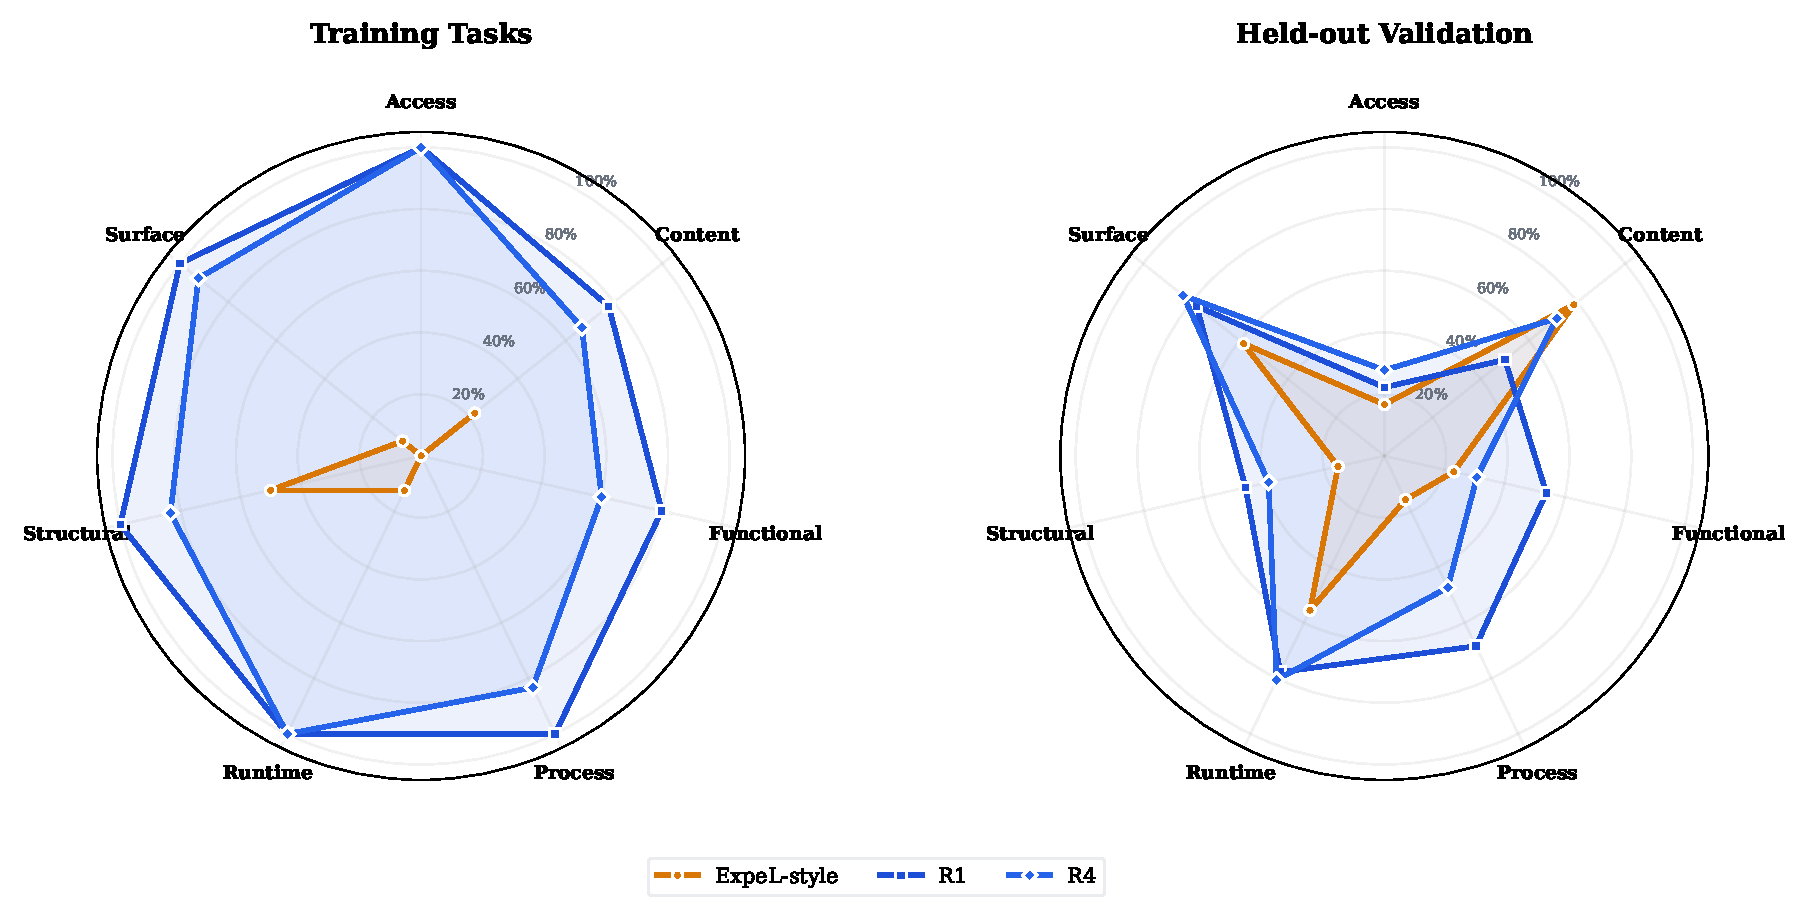
\includegraphics[width=0.95\textwidth]{output/fig3_v3_drift_rule_profile.pdf}
\caption{Per-drift website V3 success profiles for \expel{}-style rules and selected reflection-rule sets. R1 dominates the training tasks and ties the best held-out aggregate score, while R4 illustrates that a plausible later rule set can shift performance across drift families without improving the overall result.}
\label{fig:v3_drift_rule_profile}
\end{figure*}

\begin{figure*}[h]
\centering
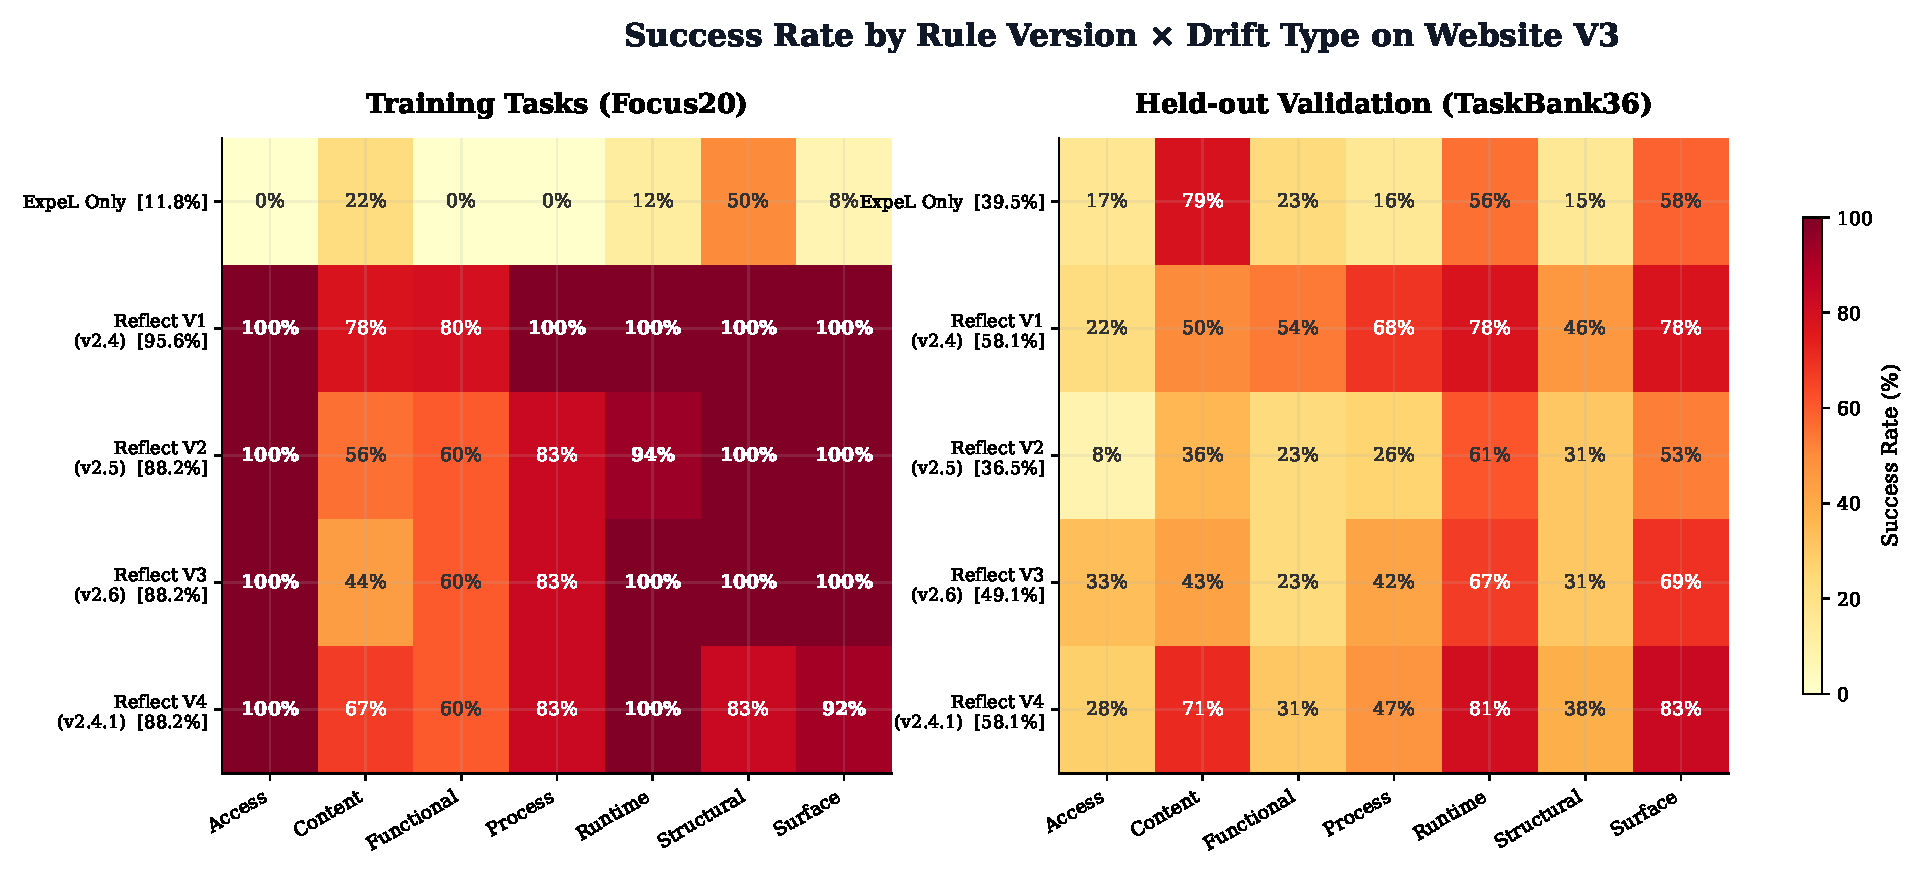
\includegraphics[width=\textwidth]{output/fig4_heatmap_rule_drift.pdf}
\caption{Full website V3 per-drift heatmap for \expel{}-style rules and all four reflection-rule sets R1--R4. This view complements the numeric tables by making drift-family regressions and improvements visually comparable across the training and held-out validation tasks.}
\label{fig:v3_rule_drift_heatmap}
\end{figure*}

\begin{figure*}[h]
\centering
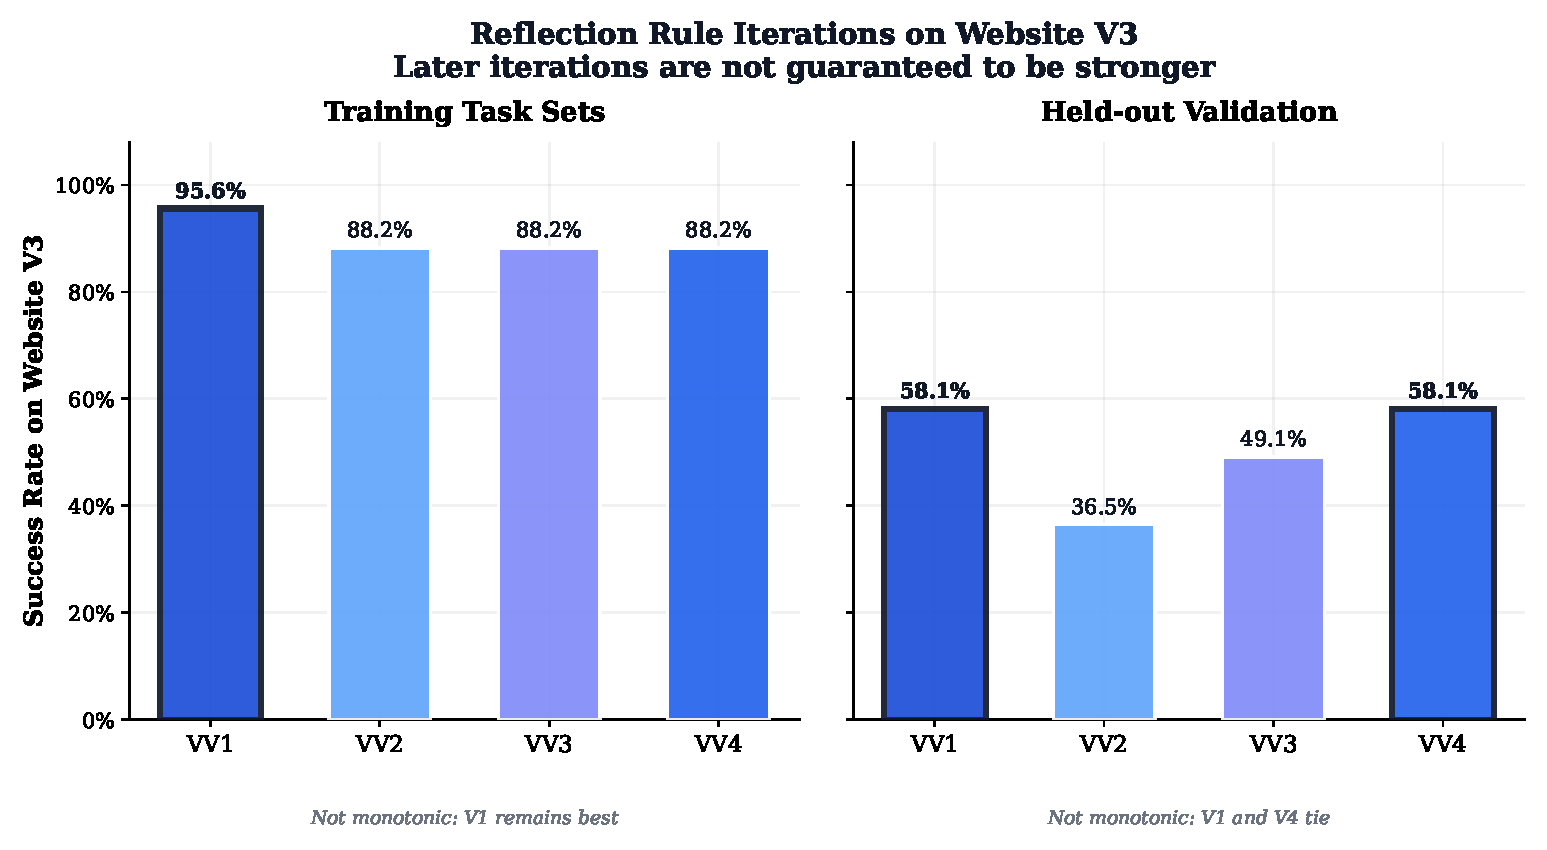
\includegraphics[width=0.9\textwidth]{output/fig2_reflection_iteration.pdf}
\caption{Aggregate website V3 performance for successive reflection-rule sets. The non-monotonic pattern supports the paper's claim that reflection-rule updates require verification before promotion.}
\label{fig:v3_reflection_iteration}
\end{figure*}

\subsection{Claim Boundary Checklist}

\begin{itemize}
\item Supported: \expel{} improves the training tasks on \linkding{} V1.45.0 from \(9/68\) to \(56/68\).
\item Supported: R1 improves over \expel{}-style rules on website V2 for both the training tasks and held-out validation tasks.
\item Supported: R1 is strongest on the training tasks under website V3 at \(65/68\).
\item Supported: R1 and R2 tie on the held-out validation tasks under website V3 at \(97/167\).
\item Not claimed: later rulebooks always improve over earlier rulebooks.
\item Not claimed: \linkding{} single-site evidence establishes broad web-agent robustness.
\item Intended next step: preserve R1's robust process/functional behavior while selectively importing R2's access/content/finalization gains.
\end{itemize}


\end{document}
